\section{Evaluation}

Die vorgestellte Methode der Texturoptimierung aus \cite{SelfTuning} wurde in MATLAB implementiert.
Die Laufzeit des Verfahrens hängt dabei von dem ausgewählten Beispielmuster und der Größe der zu synthetisierten Textur ab.
Über 33 Beispielmuster mit einer Texturgröße von $1024^2$ Pixeln auf einem 2.93GHz Intel Core i7 870 ergeben sich dabei folgende Laufzeiten (vgl. \cite{SelfTuning}):
\\

\begin{tabular}{l|rrrr}
& \textbf{Median} & Durchschnitt & Minimum & Maximum \\ \hline
Initialisierungsstrategie & \textbf{233s} & 312s & 119s & 898s \\
\glqq Guidance-Channel\grqq & \textbf{6s} & 6s & 2s & 10s \\
Texturoptimierung & \textbf{386s} & 438s & 204s & 1019s \\
\textbf{Gesamt} & \textbf{625s} & 756s & 340s & 1927s \\
\end{tabular}
\\

Zur Evaluation des Verfahrens wurden für die Beispielmuster die verschiedensten Arten von Texturen gewählt.
Diese reichen von regelmäßigen zu fast regelmäßigen und völlig unregelmäßigen Texturen über Texturen mit einer Varianz an unterschiedlich großen Details.
Abbildung \ref{examples} zeigt eine Auswahl der synthetisierten Texturen, einmal ohne und einmal mit den vorgestellten Verbesserungen.

\begin{figure}
\centering
\begin{subfigure}{0.9\textwidth}
	\centering
	\begin{subfigure}{0.3\textwidth}
		\centering
		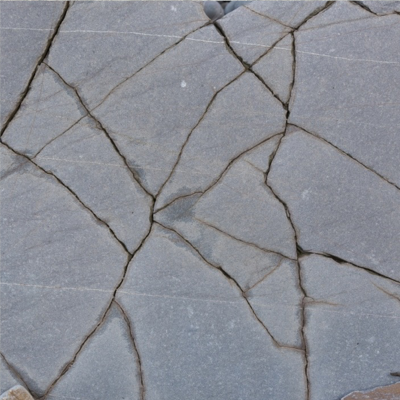
\includegraphics[width=0.6\textwidth]{images/example-1-example}
		\caption*{($a$) Beispielmuster}
	\end{subfigure}
	\hfill
	\begin{subfigure}{0.3\textwidth}
		\centering
		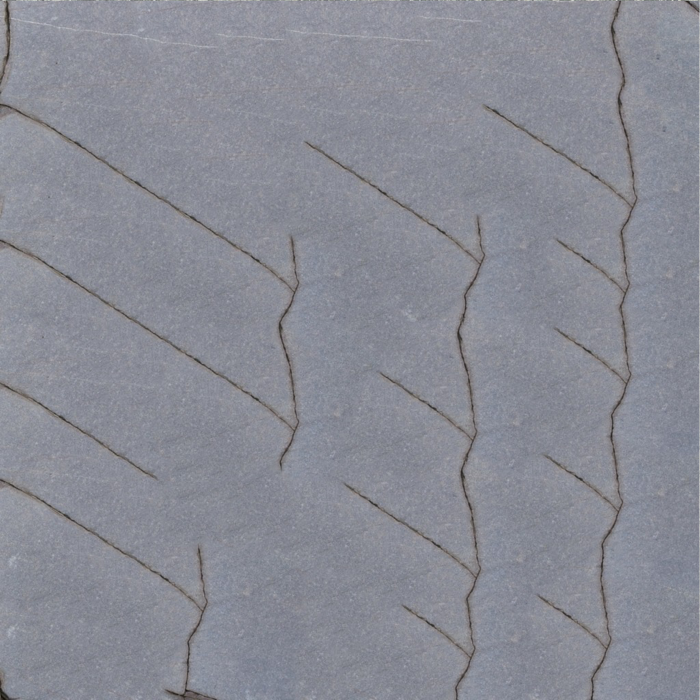
\includegraphics[width=0.9\textwidth]{images/example-1-without}
		\caption*{($b$) ohne Verbesserungen}
	\end{subfigure}
	\hfill
	\begin{subfigure}{0.3\textwidth}
		\centering
		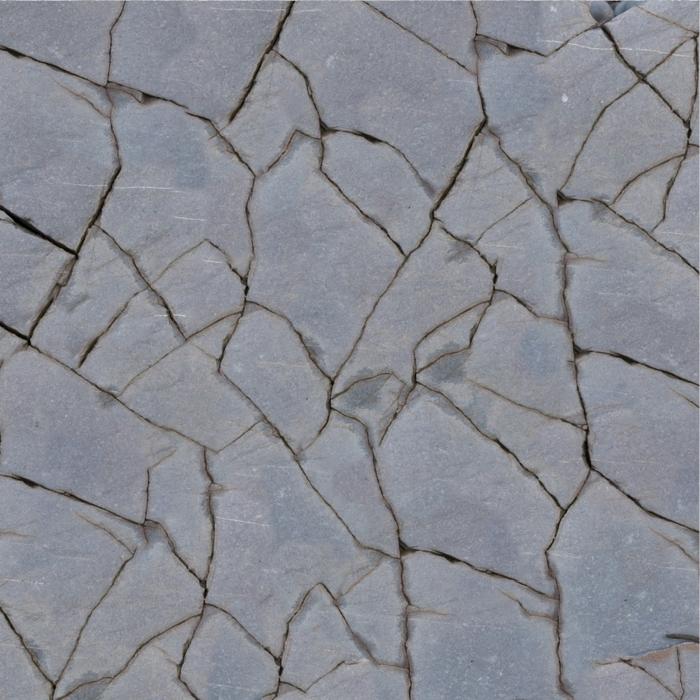
\includegraphics[width=0.9\textwidth]{images/example-1-with}
		\caption*{($c$) mit Verbesserungen}
	\end{subfigure}
	
	\caption*{($1$) Die großflächigen Strukturen des Beispielmusters bleiben in der synthetisierten Textur erhalten, wohingegen diese ohne Verbesserungen nur unzureichend repräsentiert werden.}
\end{subfigure}
\hfill
\begin{subfigure}{0.9\textwidth}
	\centering
	\begin{subfigure}{0.3\textwidth}
		\centering
		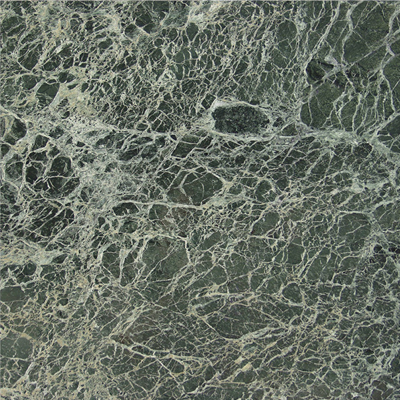
\includegraphics[width=0.6\textwidth]{images/example-2-example}
		\caption*{($a$) Beispielmuster}
	\end{subfigure}
	\hfill
	\begin{subfigure}{0.3\textwidth}
		\centering
		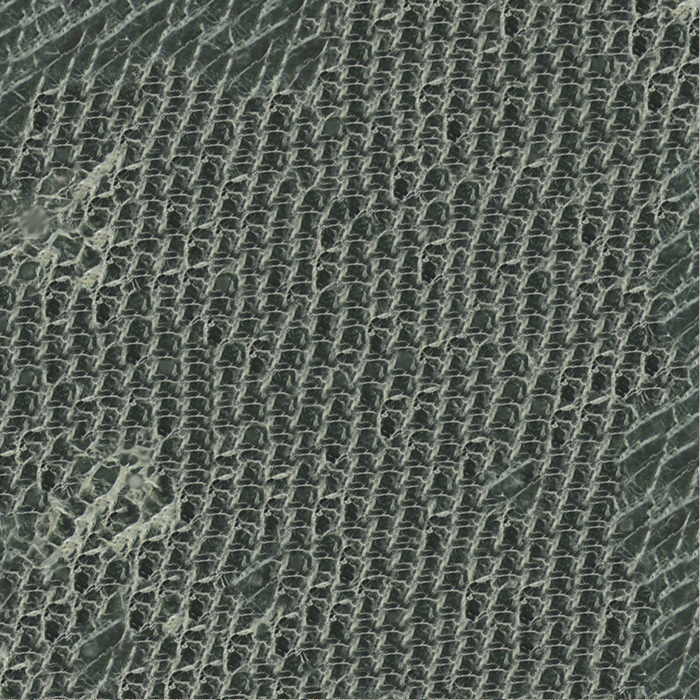
\includegraphics[width=0.9\textwidth]{images/example-2-without}
		\caption*{($b$) ohne Verbesserungen}
	\end{subfigure}
	\hfill
	\begin{subfigure}{0.3\textwidth}
		\centering
		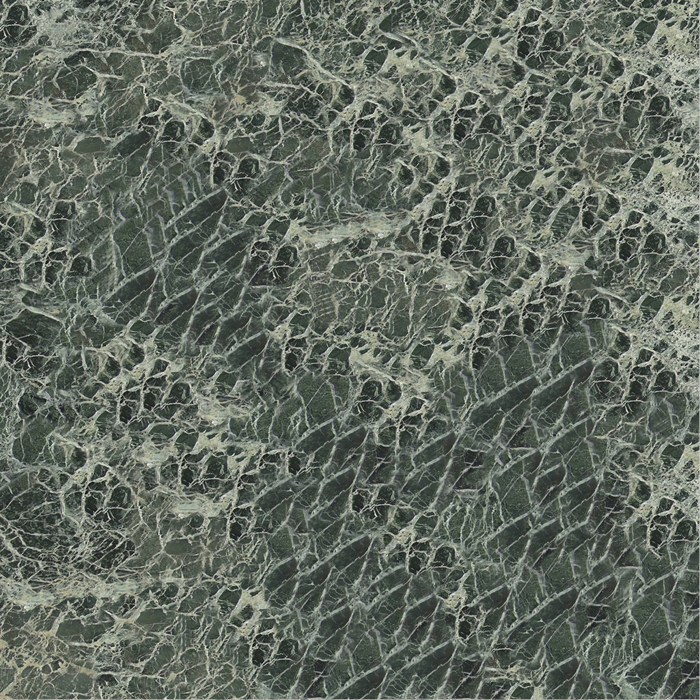
\includegraphics[width=0.9\textwidth]{images/example-2-with}
		\caption*{($c$) mit Verbesserungen}
	\end{subfigure}
	
	\caption*{($2$) Die synthetisierte Textur gewinnt mittels der Verbesserungen eine globale Ähnlichkeit zum Beispielmuster und bleibt demnach frei von auffällig sichtbaren Wiederholungen.}
\end{subfigure}
\hfill
\begin{subfigure}{0.9\textwidth}
	\centering
	\begin{subfigure}{0.3\textwidth}
		\centering
		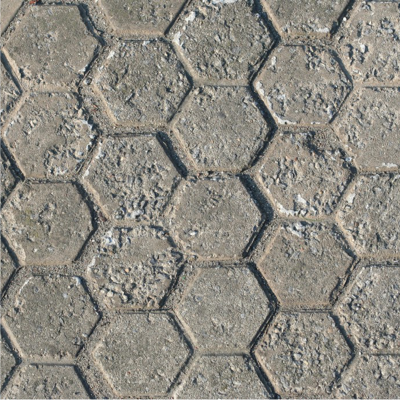
\includegraphics[width=0.6\textwidth]{images/example-3-example}
		\caption*{($a$) Beispielmuster}
	\end{subfigure}
	\hfill
	\begin{subfigure}{0.3\textwidth}
		\centering
		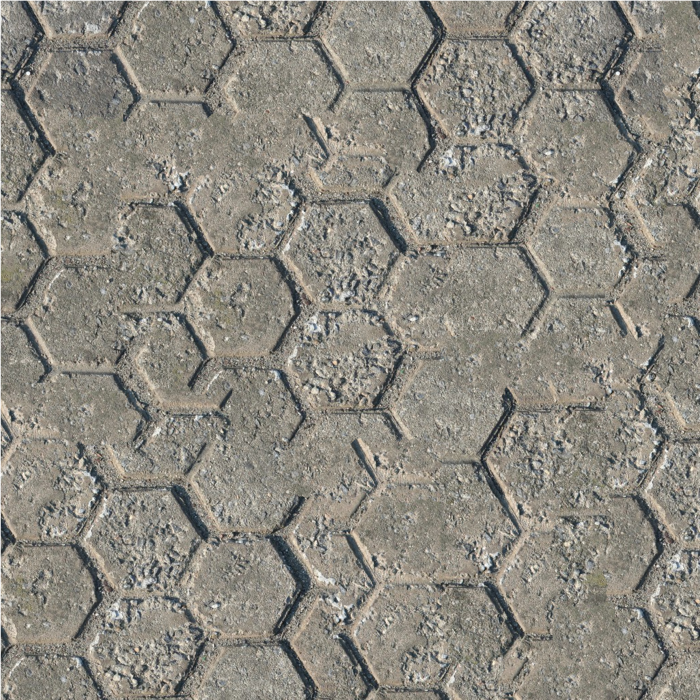
\includegraphics[width=0.9\textwidth]{images/example-3-without}
		\caption*{($b$) ohne Verbesserungen}
	\end{subfigure}
	\hfill
	\begin{subfigure}{0.3\textwidth}
		\centering
		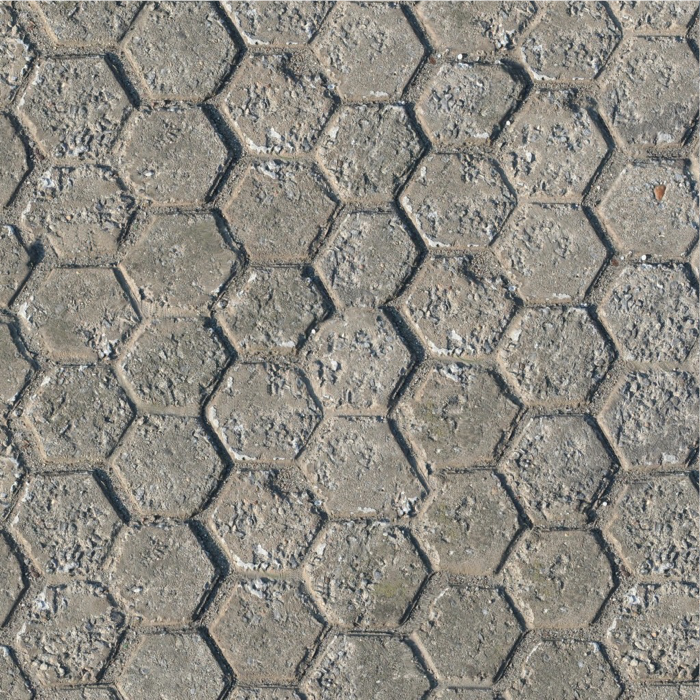
\includegraphics[width=0.9\textwidth]{images/example-3-with}
		\caption*{($c$) mit Verbesserungen}
	\end{subfigure}
	
	\caption*{($3$) Die verbesserte Textursynthese erkennt die Regelmäßigkeiten in den Steinkacheln und bewahrt diese ohne Artefakte oder Unnatürlichkeiten.}
\end{subfigure}

\label{examples}
\caption{Beispielmuster und ihre daraus synthetisierten Texturen, einmal ohne und einmal mit den vorgestellten Verbesserungen.}
\end{figure}

\cite{SelfTuning} stellen ebenso einen neuen Ansatz namens \emph{Textursequenzen} vor, um die Qualität der Ergebnisse eines Textursynthese-Verfahrens objektiv zu bewerten.
Textursequenzen bilden dabei eine Art \glqq Stress-Test\grqq.
Dafür wird die Textursynthese iterativ mit der synthetisierten Textur als Eingabe mehrfach wiederholt.
Das erlaubt die Überprüfung der Stabilität einer Textursynthese.
Regelmäßigkeiten, großflächige Strukturen und globale Ähnlichkeiten einer Textur sollen dabei im besten Fall auch über mehrere Iterationen erhalten bleiben.
Da Textursynthese-Verfahren stets einem gewissen Fehler unterliegen und dieser Fehler über das iterative Verfahren der Textursequenzen stets an die nächste Textur weiterpropagiert wird, ist auf Dauer zu erwarten, dass die erstellte Textur qualitative Abstriche in Kauf nehmen muss.
Das Verfahren aus \cite{SelfTuning} zeigt dennoch auch nach 7 Iterationen im Vergleich zu anderen Texturoptimierungen erstaunlich gute Ergebnisse (vgl. Abbildung \ref{textursequenzen}).

\begin{figure}[h]
	\centering
	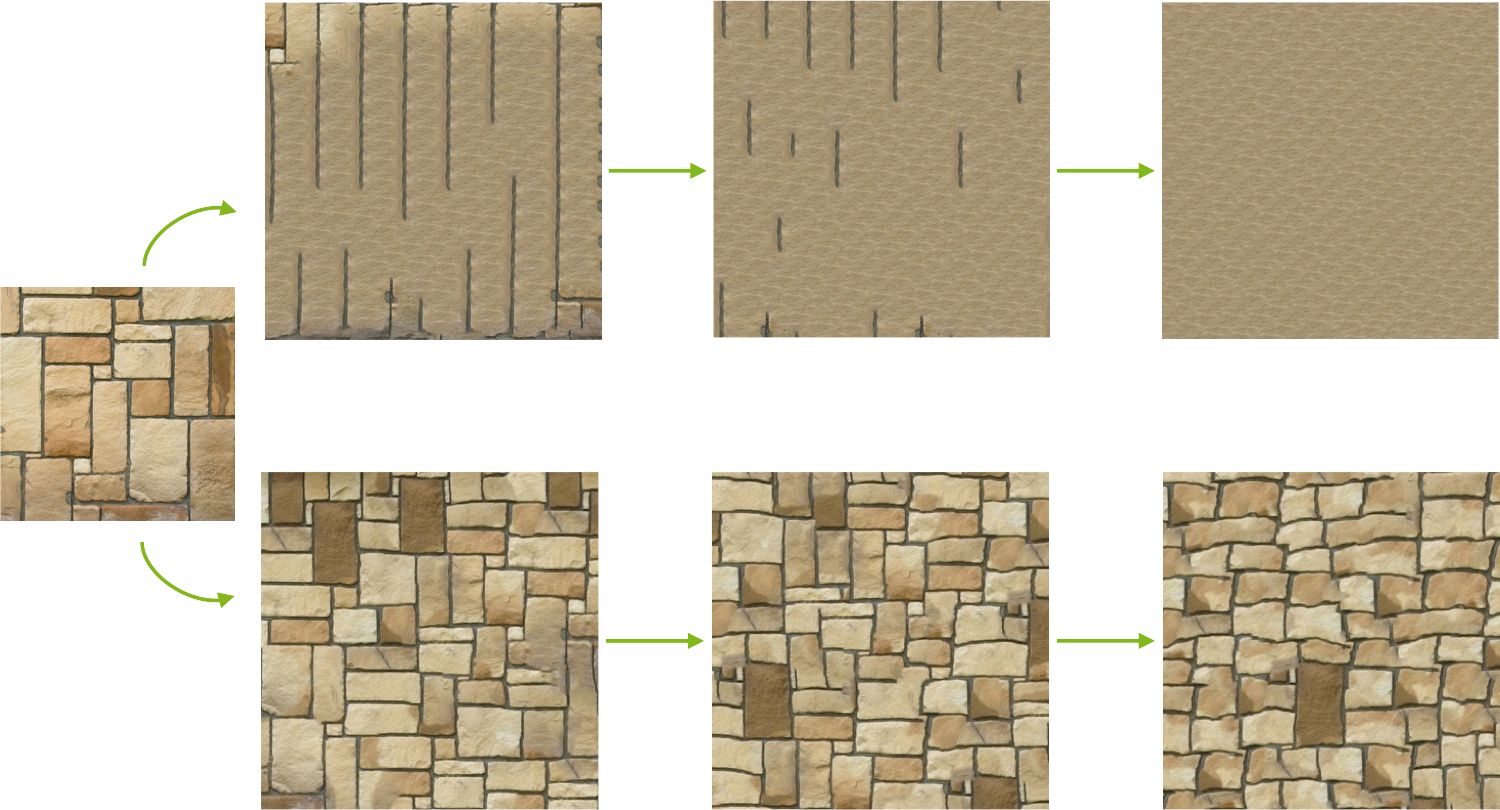
\includegraphics[width=0.9\textwidth]{images/textur-sequence-1}
	\label{textursequenzen}
	\caption{
	\glqq Stress-Test\grqq \ der Textursynthese mittels der Erstellung von Textursequenzen.
	Die Abbildung zeigt die erste, dritte und siebte Iteration der Texturoptimierung, einmal ohne (oben) und einmal mit Verbesserungen (unten).
	Die Textursynthese ohne Verbesserungen unterliegt ziemlich schnell der \glqq Markov-Random-Field\grqq -Eigenschaft und verfällt in ein Muster ohne globale Struktur.
	Die verbesserte Texturoptimierung dagegen bleibt auch nach der siebten Iteration relativ stabil.
	Unsauberkeiten zeigen sich dabei lediglich in den verformten Kanten.
	}
\end{figure}

Es ist ebenfalls anzumerken, dass das Verfahren aus \cite{SelfTuning} völlig automatisiert arbeitet und außer einem Beispielmuster und der Eingabe einer gewünschten Texturgröße keine weiteren Konfigurationsparameter von Nöten sind.
Damit ist insbesondere das Ziel erreicht, Benutzern einen einfachen aber qualitativ hochwertigen Weg für die Erstellung von Texturen zu bieten.

Obwohl mit den vorgestellten Verbesserungsmöglichkeiten bereits qualitativ hochwertige Texturen synthetisiert werden können, so bleibt dennoch genug Spielraum für weitere Verbesserungen.
So enthalten viele der synthetisierten Textur weiterhin kleine Artefakte in den Strukturen der Textur.
Es lässt sich weiterhin beobachten, dass der Kantendetektor für die Erstellung des \glqq Guidance-Channels\grqq \ einen negativen Einfluss auf Texturen mit großen, aber schwachen Kanten ausübt.
Weiterhin ist die Initialisierungsstrategie aktuell nur begrenzt auf das Erkennen einer einzigen Translationssymmetrie und erlaubt damit lediglich das Bewahren simpler Regelmäßigkeiten (vgl. \cite{SelfTuning}).